\chapter{Tecnología y Uso Sostenible del Agua}


Los retos de la agricultura son el crecimiento a nivel mundial de la demanda de alimentos; mejora de la eficiencia y protección del ambiente; innovación para ser más competitivos; calidad y seguridad alimentaria en la producción; gestión integrada de los recursos hídricos e inclusión rural.

\begin{definition}[Regulación Hídrica]
    Son aquellos que mediante acciones generan, mantienen, incrementan o mejoran la calidad, cantidad y oportunidad del recurso hídrico dentro de los parámetros requeridos para uso poblacional, riego, generación eléctrica, entre otros.
\end{definition}

\begin{example}[Operador de infraestructura hidráulica]
    Si dichos usuarios prevén en sus planes de operación, mantenimiento y desarrollo de la infraestructura hidráulica la inversión en acciones para los ecosistemas, pueden suscribir acuerdos por el servicio de regulación hídrica u otros que prioricen
\end{example}

Sin los mecanismos, empiezan una serie de cadena de producción de los servicios de saneamiento:
\begin{itemize}
    \item Captación
    \item Transporte
    \item Tratamiento de agua cruda
    \item Transporte
    \item Almacenamiento
    \item Vertimiento de aguas tratadas
    \item Transporte
    \item Plana de tratamiento de aguas residuales
    \item Redes de recolección
    \item Usuarios
    \item Redes de distribución
\end{itemize}
Es así que se incorpora un esquema de financiero para que las EPS conserve su fuente de agua

Dentro del \textbf{diseño} del plan de retribución:
\begin{itemize}
    \item Diagnóstico hídrico rápido
    \item Caracterización de Contribuyentes
    \item Sistema de monitoreo hidrológico
    \item Plan de intervenciones
    \item Plataforma de buena gobernanza
\end{itemize}

Luego está la \textbf{tarifa} 
\begin{itemize}
    \item Plan maestro optimizado
    \item Estudio tarifario
\end{itemize}

y finalmente la \textbf{ejecución}
\begin{itemize}
    \item Modalidad de ejecución
    \item Conformidad del diseño
    \item Suscripción del acuerdo
    \item Ejecución física y financiera
\end{itemize}

Las soluciones basadas en la naturaleza (SBN) están inspiradas y respaldadas por la naturaleza y utilizan o imitan los procesos naturales para contribuir a la gestión mejorada del agua.

Una SBN puede implicar la conservación o rehabilitación de ecosistemas naturales y/o la mejora o creación de procesos naturales en ecosistemas modificados o artificiales,


Se pueden aplicar a microescala (por ejemplo un inodoro seco) o a macro escala (por ejemplo un paisaje)

SbN para reducir los riesgos de eventos extremos relacionados con el agua (inundaciones y sequías)

¿A qué se refiere con soluciones basadas en la naturaleza NBS para el agua?
La seguridad hídrica tiene como objetivo es formar conocimientos, habilidades, herramientas innovadoras; capaces de realizar investigación original, de frontera y de alto nivel. En la siguiente líneas de Generación y aplicación del conocimiento:
\begin{itemize}
  \item Sistemas ambientales
  \item Hidrometeorología
  \item Sistemas Hídricos
  \item Gobernanza del agua
\end{itemize}

Los cambios en temporalidad e intensidad de precipitación, incipientes sequías y los distintos grados de desertificación han provocado que la disponibilidad de agua dulce en los países, muestre una gran heterogeneidad.
Mencionando las problemáticas, son:
\begin{itemize}
  \item Sequías más frecuentes y prolongadas
  \item Deforestación, erosión del suelo y mayor frecuencia de inundación en centros de población
  \item Escasa planeación y reducción de inversiones en el sector hídrico
  \item Altos costos de bombeo
  \item Altas pérdidas de agua en los sistemas de conducción
  \item Bajos niveles de recaudación por pago de servicio de suministro de agua
  \item Contaminación de los cuerpos de agua con los vertidos de agua residual sin tratamiento
  \item Conflictos sociales
\end{itemize}
La problemática actual:
\begin{enumerate}
    \item Sequías más frecuentes y prolongadas
    \item Deforestación, erosión del suelo y mayor frecuencia de inundación en centros de población
    \item Escasa planeación y reducción de inversiones en el sector hídrico
    \item Altos costos de bombeo
    \item Altas pérdidas de agua en los sistemas de Conducción
    \item Bajos niveles de recaudación por pago de servicio de suministro de agua+Contaminación de los cuerpos de agua con los servidos de agua residual sin Tratamiento
    \item Conflictos sociales
\end{enumerate}
% beneficio: Salud, Economía, productividad, nutrición, felicidad, integración social,

% Proyectos en parejas: Proyecto de captación de lluvia, (Video) costos, relación costos, burocracia, Mercado local, condiciones de sequía, (argumentos ventajas y desventajas) cuál de los dos proyectos tiene más viabilidad de que se construya

Alternativas productivas en SCALL
\begin{itemize}
    \item Producción de miel, de peces, (cultivos de bajos requerimientos hídricos: nopal, amaranto, coquia esteparia)
    \item Producción de cultivos de alta rentabilidad: aguacate, vainilla
    \item Especies forestales de alta rentabilidad
    \item Cercas vivas, para regular temperatura
    \item 10 a 20 cultivos en $1,200m2$ en hidroponía rustica.
\end{itemize}
\begin{figure}[h!]
    \centering
      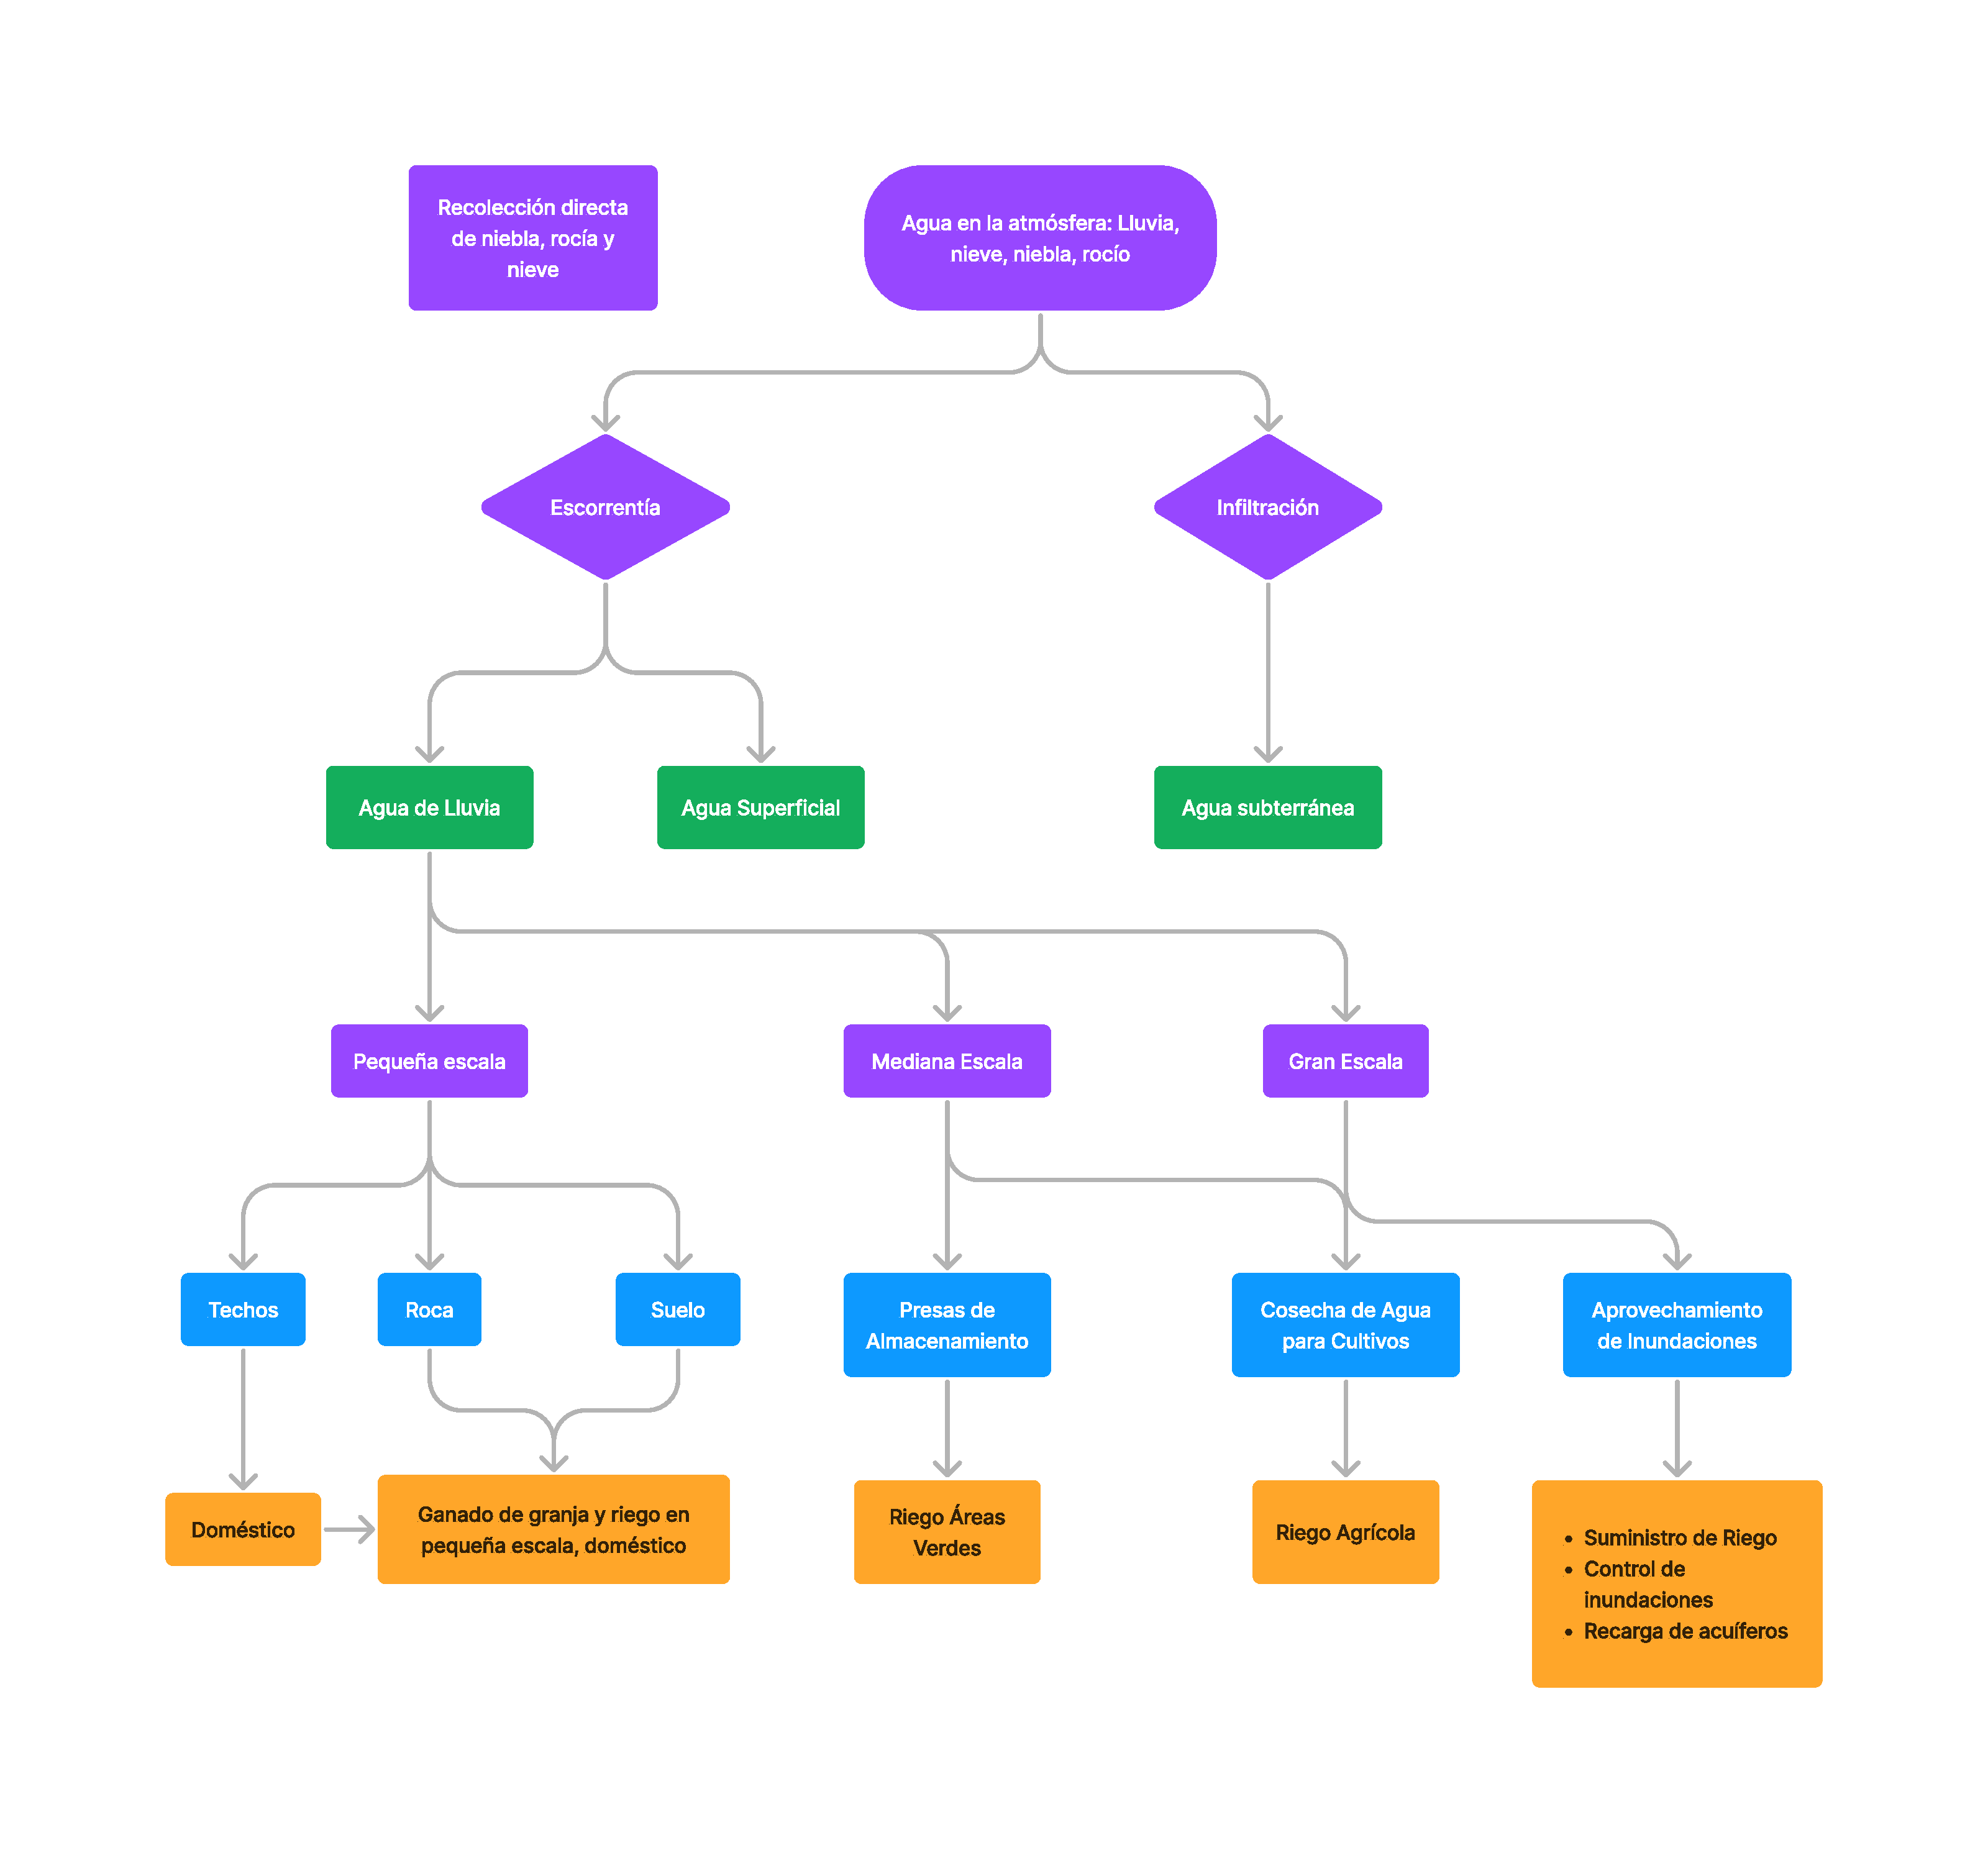
\includegraphics[width=1\textwidth]{tua1.pdf}
      \caption{Sistema de Captación de Agua de Lluvia}
      \label{tua1}
    \end{figure}
    % Fractales en las mallas atrapa nieblas con impresora 3d: Proyecto - Casa atrapanieblas y captación de agua de lluvia
    \subsection{Componentes básicos de un Sistema de Captación de agua de Lluvia}
    Está compuesto de tres componentes principales
    \begin{itemize}
        \item Área de captación
        \item Conducción
        \item Almacenamiento
    \end{itemize}
    Es importante analizar los componentes tecnológicas
    \begin{enumerate}
        \item \textbf{Área de captación:} Se refiere al techo de la vivienda para la captación de agua de lluvia. No se deben utilizar techos de asbesto, cartón, palma o algún material vegetal, ni aquellos revestidos con chapopote
        \item \textbf{Línea de conducción:} compuesta por canaletas de lámina galvanizada, tuberías y accesorios de PVC que conducirán el agua de lluvia hasta su almacenamiento
        \item \textbf{Trampa de sólidos:} Retiene las partículas sólidas que sean arrastradas por el agua de lluvia y evitar que se acumulen en la línea de conducción o en el sistema de almacenamiento
        \item \textbf{Filtro de hojas}: Retiene las partículas sólidas que sean arrastradas por el agua de lluvia y evitar que se acumulen en la línea de conducción o en el sistema de almacenamiento
        \item \textbf{Filtro de hojas:} Evita que hojas, ramas y otros objetivos lleguen a la tubería y ocasione obstrucciones o contaminación del agua almacenada
        \item \textbf{Depósito o tanque cerrado:} Mantiene el agua libre de contaminación para su posterior uso. 
\end{enumerate}
\begin{figure}[h!]
\centering
  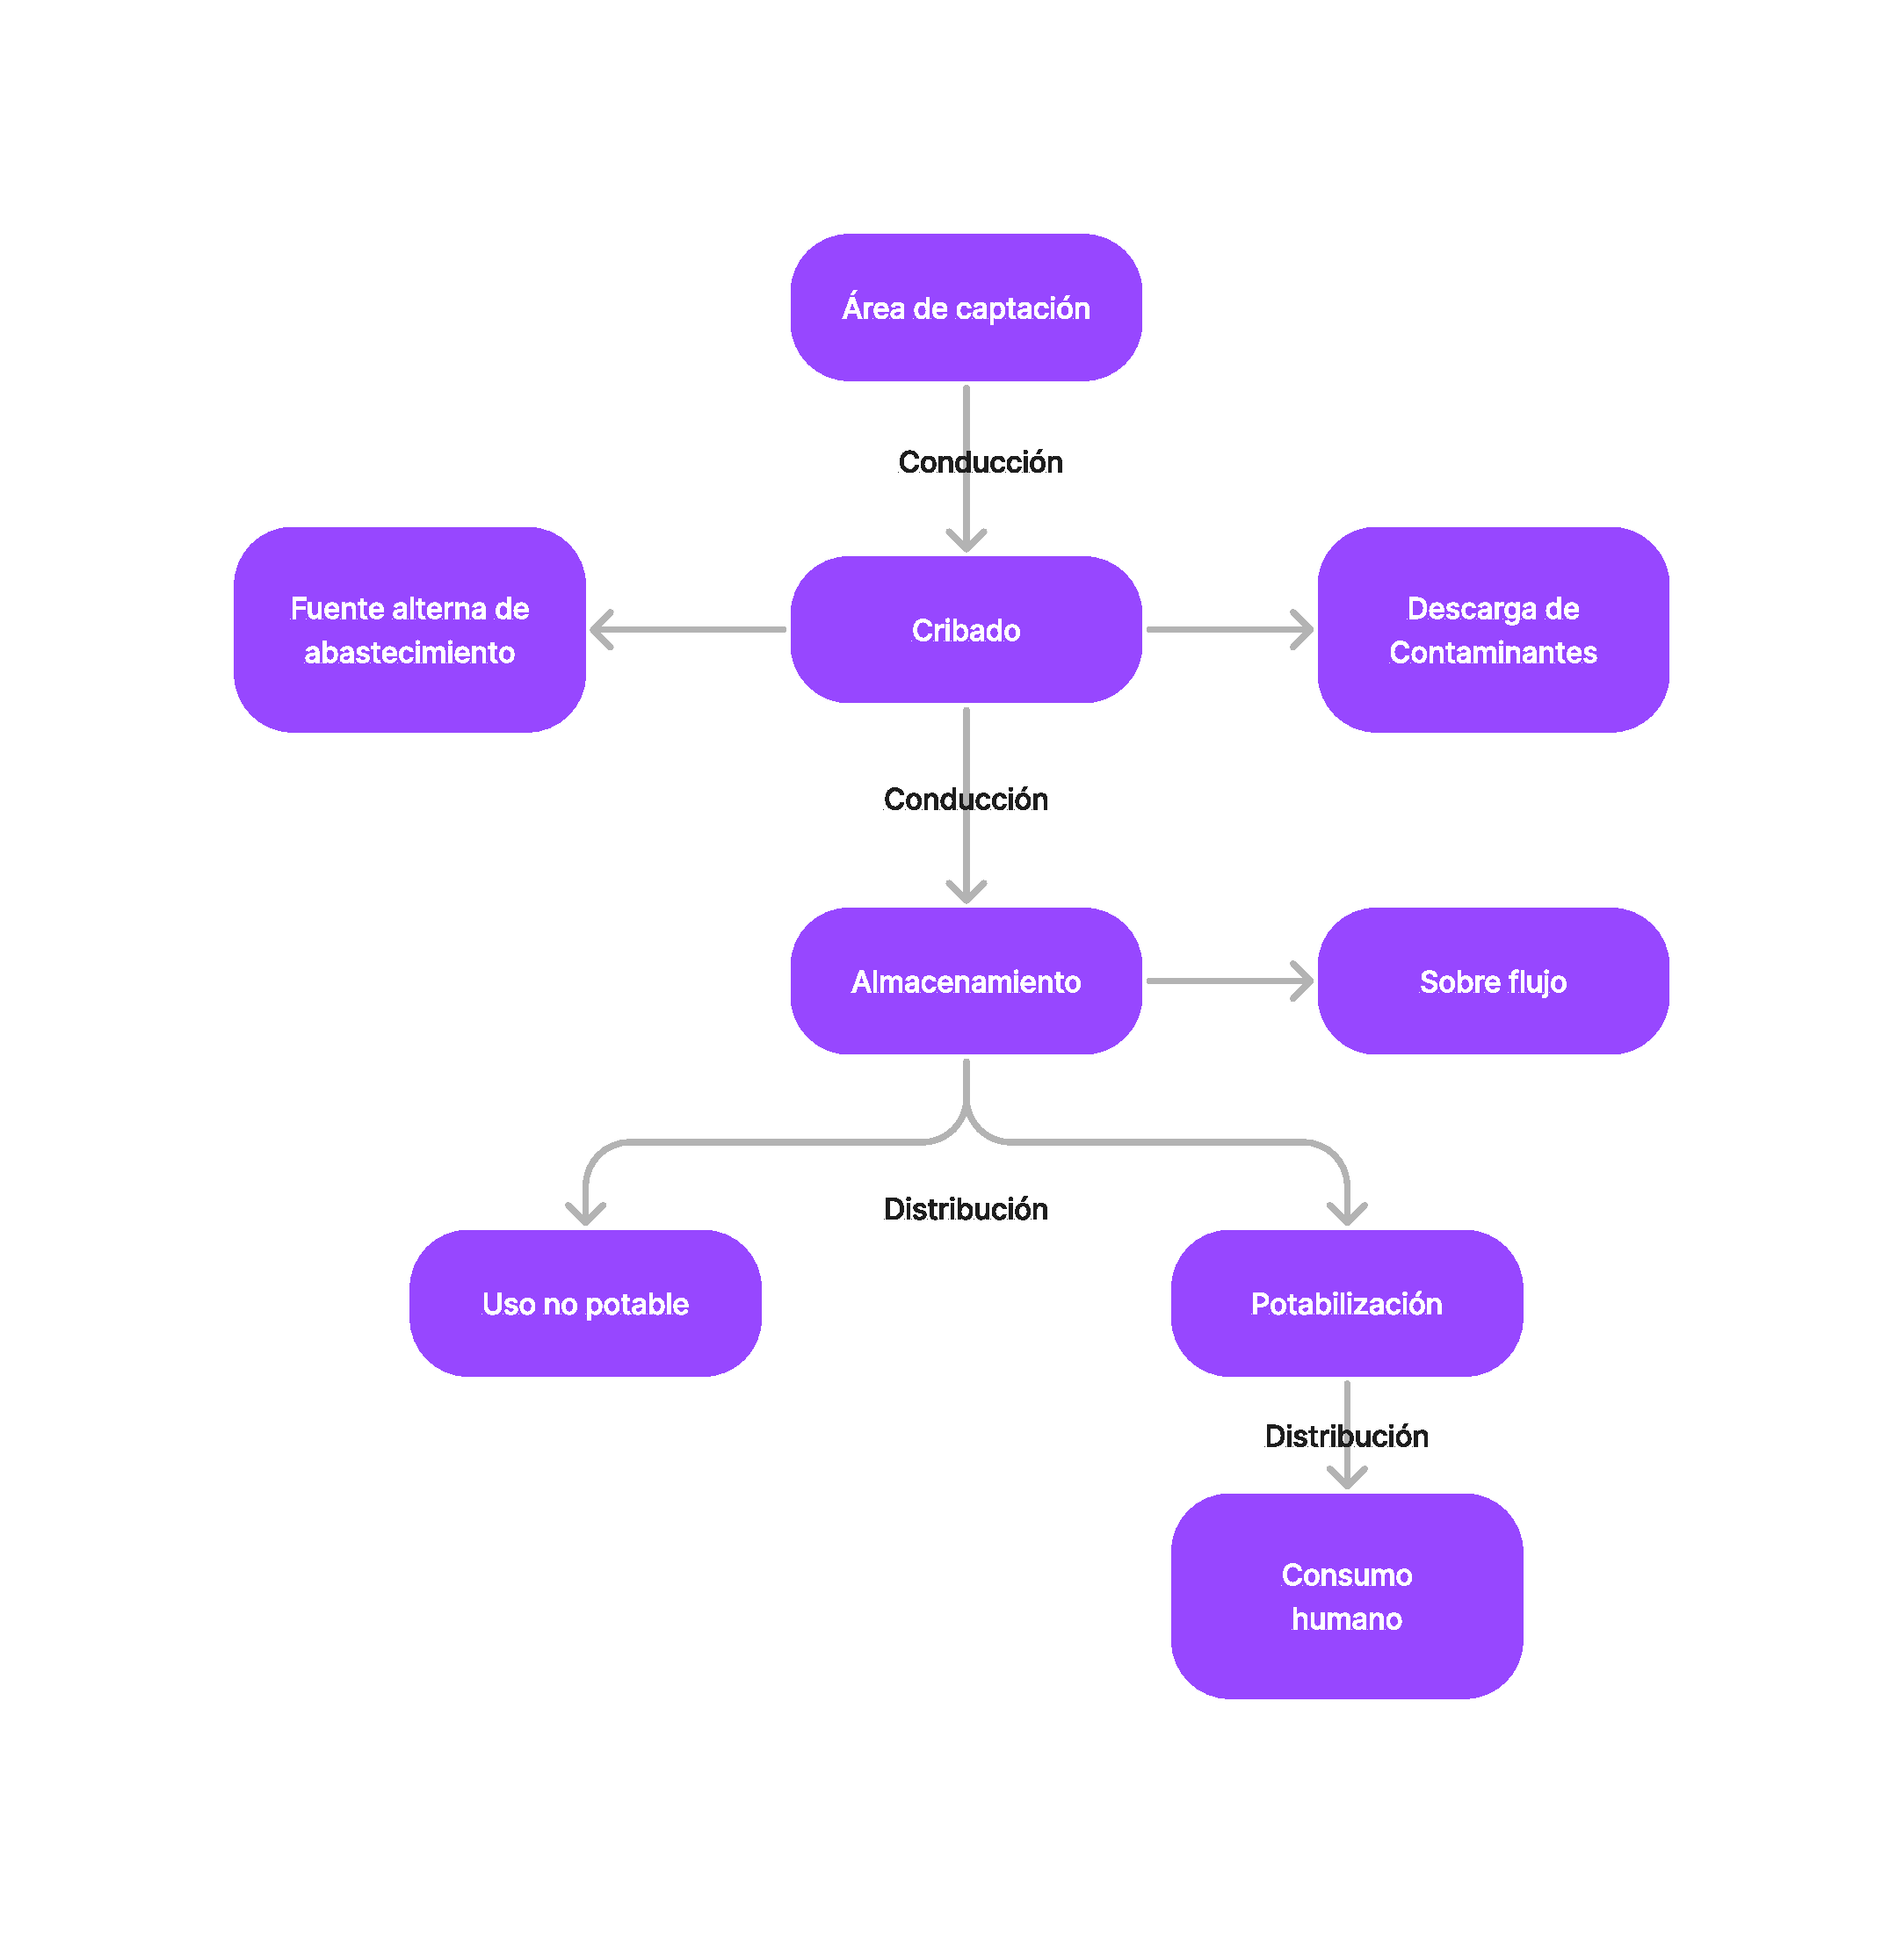
\includegraphics[width=1\textwidth]{tua2.pdf}
  \caption{Sistema de captación de agua de lluvia}
  \label{tua2}
\end{figure}
Beneficios:
\begin{itemize}
    \item Aumenta la disponibilidad de agua
    \item Disminuye la extracción de agua de los acuíferos y otras Fuentes
    \item Reduce los escurrimientos al drenaje
    \item En ligares donde el costo del agua es alto, el retorno de inversión es alto
    \item Se fomenta la cultura del uso responsable del agua
\end{itemize}
Limitaciones:
\begin{itemize}
    \item La cantidad de agua que llueve depende del lugar
    \item La lluvia es estacional, por lo que se necesitan otras fuentes de suministro
    \item El costo de implementación puede ser elevado, al inicio
\end{itemize}


    \begin{center}
        \smartdiagramset{
        set color list={blue!50!cyan,green!60!lime,orange!50!red},
        priority arrow width=2cm,
        priority arrow height advance=2.25cm
        }
        \smartdiagram[descriptive diagram]{{1,Macrolocalización del SCALL}, {2,Determinar la demanda de agua para el uso requerido}, {3,Analizar la precipitación pluvial mensual histórica y calcular la precipitación pluvial neta}, {4,Calcular el área efectiva de captación}, {5, Localizar el sitio para establecer el SCALL},{6, Diseñar el sistema d conducciones},{7,Calcular el volumen y medidas del sedimentador}, {8,Diseñar las cisternas de almacenamiento del agua de lluvia}, {9,Diseñar el sistema de bombeo (solar) del agua almacenada}, {10,Diseño del tren terciario de purificación en base de análisis del agua de lluvia}}
    \end{center}
    
    Método de ponderación de distancia inversa (IDW) o U.S. National Weather Service
    \begin{equation}
        P_x = \frac{\sum\left(P_i \cdot W_i\right)}{\sum W_i}
    \end{equation}
    \begin{notation}
        \begin{itemize}
            \item $P_x=$ Precipitación faltante estimada mm
            \item $P_i=$ Precipitación observada en la fecha faltante, en las estaciones auxiliares circundantes, mm
        \end{itemize}
    \end{notation}
    \begin{equation}
        W_i = \frac{1}{D_1^2}
    \end{equation}
    \begin{notation}
        \begin{itemize}
            \item $D_2=$ Distancia entre cada estación circundante y la estación con información faltante en km
    \end{itemize}
\end{notation}
    \begin{example}
        Obtener la precipitación pluvial media faltante del mes de enero de 1954 de la estación Higueras, a partir de los datos de las tres estaciones circundantes
    \end{example}
    \begin{table}[h!]
        \centering
        \begin{tabular}{@{}ccc@{}}
        \toprule
        Estación  & Precipitación (mm) Enero & Distancia (km) \\ \midrule
        Ciénega   & 3.5                      & 16.0           \\
        Cerralvo  & 17.8                     & 43.0           \\
        Cadereyta & 24.3                     & 45.0           \\
        Higueras  & x                        & y              \\ \bottomrule
        \end{tabular}
        \caption{Encontrar precipitación y distancia}
        \label{tabtua1}
    \end{table}
    \textit{ Sol. }
    \begin{table}[h!]
        \centering
        \begin{tabular}{@{}ccccc@{}}
        \toprule
        Estación  & Precipitación (mm) Enero & Distancia (km) & Wi              & P*W            \\ \midrule
        Ciénega   & 3.5                      & 16             & 0.00390625      & 0.013671875    \\
        Cerralvo  & 17.8                     & 43             & 0.0005408328826 & 0.009626825311 \\
        Cadereyta & 24.3                     & 45             & 0.0004938271605 & 0.012          \\
        Higueras  & x                        & y              &                 &                \\
        SUMA      &                          &                & 0.004940910043  & 0.03529870031  \\ \bottomrule
        \end{tabular}
        \caption{Cálculos del problema}
        \label{tabtua2}
\end{table}
Por ultimo, la ecuación queda:
\begin{equation*}
    P_x=\frac{\sum P\cdot W}{\sum W_i} =\frac{0.03529870031}{0.004940910043} = 7.1441
\end{equation*}

\subsubsection{Módulo de captación de aguas de lluvia}

Con base en diagnósticos previos y en reuniones con los habitantes de la microcuenca seleccionada se determinaron los usuarios participantes en la construcción de los módulos de captación. Una de las características elegidas en los beneficiarios es el interés mostrado y la participación en las actividades que se realizarían.

La ecotecnia denominada Módulo de captación de Agua de Lluvia, es una opción desde el punto de vista técnico y económico para el aprovechamiento de la lluvia para uso doméstico en el medio rural y zonas urbanas, siendo esencialmente ecológica.
\subsection{Cálculo de la precipitación pluvial de diseño}
Se debe estimar la precipitación de la zona de estudio y calcular la precipitación pluvial de diseño mediante el CIDECALLI (CP), UNASABAR y con probabilidad.

\subsubsection{Metodología de CIDECALLI}
\begin{equation}
    P_{dis} = PN \cdot Ce \cdot C_c
\end{equation}
\begin{notation}
\begin{itemize}
    \item $PN=$ Precipitación neta en mm
    \item $Ce=$ Coeficiente de escurrimiento adimensional
    \item $Cc=$Coeficiente de captación adimensional
\end{itemize}
\end{notation}
Se propone un valor empírico de 0.85 por las pérdidas de salpicamiento, velocidad del viento, evaporación, fricción y tamaño de gota.
En el caso del escurrimiento, véase la tabla
\begin{table}[h!]
    \centering
    \begin{tabular}{@{}cc@{}}
    \toprule
    Tipos de captación                   & $Ce$           \\ \midrule
    \textbf{Cubiertas superficiales}     &                \\
    Concreto                             & 0.6-0.8        \\
    Pavimento                            & 0.5-0.6        \\
    Geomembrana de PVC                   & 0.85-0.90      \\
    \textbf{Azotea}                      &                \\
    Azulejos, teja                       & 0.8-0.9        \\
    Hojas de metal acanaladas            & 0.7-0.9        \\
    Orgánicos (hojas con barro)          & \textless{}0.2 \\
    \textbf{Captación en tierra}         &                \\
    Suelo con pendientes menores al 10\% & 0.0-0.03       \\
    Superficies naturales rocosas        & 0.2-0.5        \\ \bottomrule
    \end{tabular}
    \caption{Coeficientes de escurrimiento (Ce) de los diferentes materiales en el área de captación}
    \label{tabtusa1}
\end{table}
\begin{table}[h!]
    \centering
    \begin{tabular}{@{}cc@{}}
    \toprule
    Metales del techo         & Coeficiente de escurrimiento \\ \midrule
    Lámina galvanizada lisa   & \textgreater{}0.9            \\
    Lámina metálica corrugada & 0.7-0.9                      \\
    Lámina de asbesto         & 0.8-0.9                      \\
    Teja                      & 0.6-0.9                      \\
    Palma                     & 0.2                          \\ \bottomrule
    \end{tabular}
    \caption{Coeficientes de escurrimiento de agua de lluvia para techos de varios materiales. Lee y Visscher (1992) y caballero (2007)}
    \label{tabtusa2}
\end{table}

$PN$ es la suma de los meses que tengan más de 40mm.

% media: 170
% desv : 12
% mayores de 145
% Tabla de distribución: 98.12
% ¿Qué estatura deja por debajo de si al 80\% de la población?
% z=-2.0833
% Tablas de z el que este .8
% 0.84-79.95 | 180

% Estimar la precipitación mensual con un 80\% de probabilidad

\section{Captación de Agua de Lluvia}
\begin{equation}
    P(\%) = \frac{m - 0.375}{N + 0.25} \cdot 100 
\end{equation}
\begin{notation}
\begin{itemize}
    \item $P$ Probabilidad \%
    \item $M$ número de orden
    \item $N$ Número total de observaciones
\end{itemize}
\end{notation}
Establecer las bases para el diseño y ejecución de proyectos sobre sistemas de captación y aprovechamiento del agua de lluvia para consumo humano, uso doméstico, consumo animal e irrigación.

Para determinar la demanda de agua, es la cantidad de agua requerida para satisfacer la necesidad establecida en el objetico del proyecto

La expresión matemática para calcular la demanda de agua es la siguiente:
\begin{align}
    &D_j =\frac{Nu \cdot Dot \cdot Nd_j}{1000}\\
    &D_{anual} =\sum_{j = 1}^{12}\\
\end{align}
\begin{notation}
    \begin{itemize}
        \item $D_j$ Demanda de agua en el mes $j$, $m^3/mes/poblacion$
        \item $Nu$ Número de beneficios del sistema
        \item $Dot$ dotación en l/persona/día
        \item $Nd_j$ Número de días del mes $j$,
        \item $D_{anual}$ demanda de agua para la población
        \item $j$ Número del mes $j=1,2,3$
        \item 1000 factor de conversión de litros a $m^3$
    \end{itemize}
\end{notation}
\begin{example}
    El requerimiento de agua para consumo humano se calcula considerando el 3\% del peso corporal (OMS)

    ¿Cuál es el requerimiento de agua para consumo humano de una persona con un peso de 80kg?

    \textit{ Sol. }

    2.4L/día

    Para fines prácticos se estima 1 $m^3$/persona/año, equivalente a 2.73 L/persona(día) (OMS)
\end{example}

\begin{problem}[¿Cuál es la demanda de agua para satisfacer el consumo humano de una familia de 4 integrantes de marzo a julio? Considerar un requerimiento de agua de 100L/personas/día]
    
    \textit{ Sol. }

    100L/día/persona*4 personas*153 días =$61.3m^3$
\end{problem}
\begin{table}[h!]
    \centering
    \begin{tabular}{@{}ccc@{}}
    \toprule
    \begin{tabular}[c]{@{}c@{}}Nivel de complejidad\\ del sistema\end{tabular} &
      \begin{tabular}[c]{@{}c@{}}Dotación neta\\ (L/hab*día)\\ climas templado y frío\end{tabular} &
      \begin{tabular}[c]{@{}c@{}}Dotación neta\\ (L/hab*día)\\ clima cálido\end{tabular} \\ \midrule
    Bajo       & 90  & 100 \\
    Medio      & 115 & 125 \\
    Medio alto & 125 & 135 \\
    Alto       & 140 & 150 \\ \bottomrule
    \end{tabular}
    \caption{Dotación}
    \label{tabtusa3}
\end{table}

\begin{table}[h!]
    \centering
    \begin{tabular}{@{}cc@{}}
    \toprule
    Tipo de instalación        & Consumo de agua    \\ \midrule
    Educación elemental        & 20L/alumno/jornada \\
    Educación media y superior & 25L/alumno/jornada \\ \bottomrule
    \end{tabular}
    \caption{Dotación en escuelas}
    \label{tabtusa4}
\end{table}

\begin{example}
    ¿Cuál es la demanda de agua para satisfacer el requerimiento de 50 gallinas de 1.3kg durante un año? Considerar un requerimiento de agua de 0.3 L/día/gallina
    \textit{ Sol. }
    
    0.3L/día/gallina*50 gallinas*365 días=$5.475m^3$
\end{example}

\subsection{Demanda de agua en riego}
Requerimiento de agua de un cultivo, evapotranspiración de cultivo ($Et_c$), la demanda de agua considerará la eficiencia de riego.
\begin{equation}
    RR = ET_c - Pe
\end{equation}
\begin{notation}
    \begin{itemize}
        \item $RR$ Requerimientos de riego
        \item $ET_c=ET_o*k_c$ Evapotranspiración
        \item $Pe$Transpiración efectiva
        \item $ET_o$ Evaporación del cultivo de referencia
    \end{itemize}
\end{notation}
\begin{problem}[Requerimientos de riego del cultivo de frijol, en 100 días cuando se necesia $3litros/m^2$ en una hectárea]
    \textit{ Sol. }
    \begin{equation}
        \frac{\frac{3L}{m^2}*100*10,000m^2}{1,000L} = 3000m^3
    \end{equation}
\end{problem}
\begin{table}[h!]
    \centering
    \begin{tabular}{@{}llrrr@{}}
    \toprule
    \multicolumn{2}{l}{\multirow{2}{*}{Zona climática}} &
      \multicolumn{1}{l}{Temperatura media diaria ($^{\circ}C$)} &
      \multicolumn{1}{l}{} &
      \multicolumn{1}{l}{} \\ \cmidrule(l){3-5} 
    \multicolumn{2}{l}{} &
      \multicolumn{1}{l}{\begin{tabular}[c]{@{}l@{}}Fría\\ 10\end{tabular}} &
      \multicolumn{1}{l}{\begin{tabular}[c]{@{}l@{}}Moderada\\ 20\end{tabular}} &
      \multicolumn{1}{l}{\begin{tabular}[c]{@{}l@{}}Caliente\\ \textgreater{}30\end{tabular}} \\ \midrule
    \multirow{2}{*}{Trópico y subtrópico} & Húmedo y subhúmedo & 2-3 & 3-5 & 5-7 \\
                                          & Semiárido y árido  & 2-4 & 4-6 & 6-8 \\
    \multirow{2}{*}{Regiones templadas}   & Húmedo y subhúmedo & 1-2 & 2-4 & 4-7 \\
                                          & Semiárido y árido  & 1-3 & 4-7 & 6-9 \\ \bottomrule
    \end{tabular}
    \caption{Valores de referencia de ETO, Allen 2006}
    \label{tabtusa5}
\end{table}
La ecuación \eqref{eqtusa1}, es de la FAO  por Penmann-Monteith, derivada de la ecuación original, para el cálculo de la $ETo$, la cual presenta buena capacidad de reproducción de la realidad.
\begin{equation}
\label{eqtusa1}
    Eto = \frac{0.408\Delta\left(R_n - G\right) +\frac{\zeta \cdot 900U_2\left(e_s - e_a\right)}{T + 273}}{\Delta +\zeta\left(1 + 0.34U_2\right)}
\end{equation}
\begin{notation}
    \begin{itemize}
        \item $Eto$ Evapotranspiración de referencia (mm día$^{-1}$)
        \item $\Delta$ Pendiente de la curva de presión de vapor ($kPa^{\circ}C$)
        \item $Rn$ Radiación neta en la superficie del cultivo $(kPa^{\circ}C^{-1})$
        \item $G$ Flujo de calor en el suelo
        \item $T$ Temperatura media del aire a 2m de altura $^{\circ}C$
        \item $U_2$ Velocidad del viento a 2m de altura ($m s^{-1}$)
        \item $e_s$ Presión de vapor $(kPa)$
        \item $e_a$ Presión real de vapor $(kPa)$
        \item $e_s-e_a$ Déficit de presión de vapor $(kPa)$
        \item $\zeta$ Constante psicométrica ($kPa^{\circ}C^{-1}$)
    \end{itemize}
\end{notation}

Métodos para estimar $ETo$ son:
\begin{itemize}
    \item Blaney-Criddle
    \item Thornwaite
    \item Radiación
    \item Hargreaves
    \item Penman
    \item Penman-Monteith
\end{itemize}
Los métodos para estimar $Pe$ son:
\begin{itemize}
    \item Porcentaje fijo
    \item USDA
    \item Blaney-Criddle
\end{itemize}
Los métodos para estimar $Kc$
\begin{itemize}
    \item USA
    \item Grassi-Christiansen
    \item Hasen
    \item FAO (1990)
\end{itemize}
\begin{equation}
    \frac{\text{Necesidad de agua de las plantas - lluvia de diseño}}{\text{Lluvia de diseño}\times\text{Coeficiente de escorrentía}\times\text{Factor de eficiencia}}=\frac{\text{Area de captación}}{\text{Area Cultivada}}
\end{equation}
$0.1\leq$ coeficiente de escorrentía $\leq 0.5$ y $0.5\leq$ Factor de eficiencia de escurrimiento $\leq 0.75$

% Lluvia de diseño
% \begin{equation}
%     \text{Lluvia de diseño}=0.5 \cdot \left(\right) +
% \end{equation}
\subsubsection{Cálculo del depósito}
\begin{definition}[Diseño Hidrológico]
    Análisis de la precipitación de diseño y las pérdidas
\end{definition}
\begin{definition}[Diseño Constructivo]
    Dimensionar la balsa de almacenamiento; materiales de la zona de captación y cisterna
\end{definition}
\begin{definition}[Tratamiento de agua]
    El uso de riego, para potabilizar o animales
\end{definition}
\begin{equation}
    Ac = \frac{V_T}{C \cdot P_m}
\end{equation}
\begin{notation}
\begin{itemize}
    \item $AC$ Área de captación $m^2$
    \item $V_T$ volumen de la estructura
    \item $C$ Coeficiente de escorrentía
    \item $P_m$ Precipitación promedio anual
\end{itemize}
\end{notation}
\begin{example}
    Consumo humano estimado por persona por día: 25 litros; número de personas en la vivienda: 5; precipitación media anual $P\%=360mm$; Coeficiente de escorrentía del techo:0.70; número de días de uso del agua: 365;
    \textit{ Sol. }

    El consumo anual es: $25*5*365=46.625L=VT$, de manera que:
    \begin{equation*}
        A_c=\frac{45.625}{\left(0.70\right)**\left(360\right)}=181m^2
    \end{equation*}
\end{example}
\begin{equation}
    A_{ec} =\frac{D_{anual}}{\sum_{j = 1}^{12}\bar{P}N_j}
\end{equation}
\begin{notation}
\begin{itemize}
    \item $A_{ec}$ Es el área de captación necesaria para abastecer la demanda de agua a una familia o comunidad en $m^2$
    \item $D_{anual}$ Demanda anual de agua que necesita una población
    \item $\sum_{j = 1}^{12}\bar{P}N_j$ Suma de las precipitaciones netas medias mensuales que originan el escurrimiento, mm
\end{itemize}
\end{notation}
\begin{equation}
    A_c =\frac{D_{anual}}{P_{dis}}
\end{equation}
\begin{notation}
\begin{itemize}
    \item $A_c$ Es el área de captación $m^2$
    \item $D_{Anual}$ Demanda anual, $m^3$
    \item $V_{captado}$ Volumen anual captado, $m^3$
    \item $P_{dis}$ Precipitación de diseño, m
\end{itemize}
El coeficiente de escurrimiento para geomembrana es $Ce=0.85$ y la $V_{captado}=A_c\cdot P_{dis}$
\end{notation}
\begin{example}
    Para un cultivo de frijol en una hectárea, tenemos una $D_{anual}= 340.6-115.8=224.8mm$ 
    lo cuál es $\frac{2248}{E_a} m^2$

    \textit{ Sol. }
    \begin{align*}
        &P_N = 155.8mm = 0.1558m\\
        &P_{dis} = P_N \cdot C_e = 0.1558 \cdot 0.85 = 0.13243m\\
        &A_c =\frac{2248m^2}{0.13243m} = 16,975.0m^2\implies L = 130.3
    \end{align*}
\end{example}
Las recomendaciones son que el tirante normal del orden del 60\% de la altura de la canaleta; la velocidad del orden de $1.0m/s$; pendiente del orden de 1\% a 3\% y el área transversal total de la canaleta se divide entre 4.
\begin{figure}[h!]
\centering
  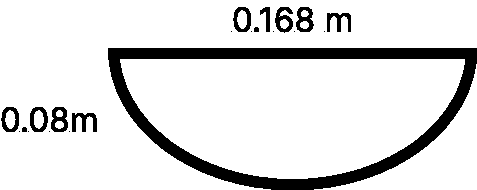
\includegraphics[width=0.5\textwidth]{tusa3.pdf}
  \caption{Dimensiones de la canaleta}
  \label{tusa3}
\end{figure}
\subsubsection{Caudal recolectado}
De una estación meteorológica con una precipitación máxima diaria de 120.9 mm, se usa la tabla \ref{tabtusa6}, se usaría $I=120.9*0.3=36.26$. 
\begin{table}[h!]
    \centering
    \begin{tabular}{@{}cccccccccc@{}}
    \toprule
    1   & 2    & 3    & 4    & 5    & 6    & 8    & 12  & 18  & 24 \\ \midrule
    0.3 & 0.39 & 0.46 & 0.52 & 0.57 & 0.61 & 0.68 & 0.8 & 0.9 & 1  \\ \bottomrule
    \end{tabular}
    \caption{Valores para las relaciones a la lluvia de duración 24 horas (Datos tomados de Campos 1978)}
    \label{tabtusa6}
\end{table}
Si se usa la ecuación \eqref{eqtusa2}, entonces $I=54.62mm/hr$
\begin{equation}
    P = P_{245h}\left(\frac{D}{1440}\right)^{0.25}
    \label{eqtusa2}
\end{equation}
Y su el área de captación es $100m^2$, entonces mediante la ecuación \eqref{eqtusa2}, le gasto es $0.14lps$
\begin{equation}
    Q =\frac{P {\max} \cdot A_c}{24 \cdot 3600}
    \label{eqtusa3}
\end{equation}
\begin{notation}
    \begin{itemize}
        \item $P_{max}-$lluvia: $Q-lps$
        \item máxima diaria, mm: $A_c-m^2$
    \end{itemize}
\end{notation}
Datos de la tabla \ref{tabtusa6}, de la precipitación normal y máxima diaria.
\begin{equation}
    Q = \frac{5}{18} \cdot \left(I \cdot A_c\right)
\end{equation}
La cuál viene de la ecuación del gasto $Q=\frac{A}{n}r^{2/3}S^{1/2}$
\begin{equation}
    I = a \cdot \frac{T^b}{t^c} \cdot M^d
\end{equation}
Por lo tanto la intensidad:
\begin{align*}
    &I=\frac{160 \cdot \sqrt{T}}{t^{0.46}}\\
    &I = 39.9532 \cdot \frac{T^{0.209014}}{t^{0.61885}}
\end{align*}
\begin{equation}
    Q = C \cdot T \cdot 0.00618 \cdot \left(P_{24}^T\right)^{1.24} \cdot A_P^{0.88}
\end{equation}
\begin{notation}
    \begin{itemize}
        \item $Q$ Es el caudal instantáneo máximo asociado al periodo de retorno $T$ años en $m^3/s$
        \item $C(T)$ Es el coeficiente empírico de periodo de retornen $T$ años
        \item $P_{24}^T$ Es la precipitación diaria máxima asociada al periodo de retorno de T años en mm
        \item $A_P$ es el área pluvial de la cuenca en $km^2$
    \end{itemize}
\end{notation}
Según Verni King el gasto es:
\begin{align*}
    &Q = 0.001854T^{0.19}\left(P_{\max }^{T}\right)^{1.24}A_c^{0.88}\\
    &C(T) = 0.3T^{0.19}\\
    &Q = 0.0002778 \cdot Ce \cdot I_{5.10} \cdot A_c
\end{align*}
\begin{equation}
    t_c = 3.98\left(\frac{L}{S^{0.5}}\right)^{0.77}
\end{equation}
\begin{notation}
    \begin{itemize}
        \item $t_c$ Tiempo de concentración (minutos)
        \item $L$ Longitud del cauce (km)
        \item $S$ Pendiente media (m/m)
    \end{itemize}
\end{notation}
\subsubsection{Caudales máximos permisibles en bajantes pluviales}
\begin{table}[h!]
    \centering
    \begin{tabular}{@{}cc@{}}
    \toprule
    Diámetro mm (pulg) & Caudal máximo (lps) \\ \midrule
    50(2)              & 0.90                \\
    75(3)              & 2.50                \\
    100(4)             & 5.10                \\
    Rectangular 60*101 & 3.75                \\ \bottomrule
    \end{tabular}
    \caption{Código de instalaciones mexicanas CFIA (Colegio federado de ingenieros y arquitectos de Costa Rica)}
    \label{tabtusa7}
\end{table}

\begin{align*}
    &D = \sqrt{\frac{4Q}{\pi V}}\\
    &D = 0.66\left[e^{1.25}\left(\frac{LQ^2_c}{gh_L}\right) + vQ_c^{9.4}\left(\frac{L}{gh_L}\right)^{5.2}\right]^{0.04}
    &h_L = f\cdot \frac{LV^2}{2g\cdot D}
\end{align*}
\begin{table}[h!]
    \centering
    \begin{tabular}{@{}cccc@{}}
    \toprule
    \multirow{2}{*}{\begin{tabular}[c]{@{}c@{}}Diámetro\\ exterior\\ nominal\\ (mm)\end{tabular}} &
      \multicolumn{3}{c}{\begin{tabular}[c]{@{}c@{}}metro de \\ recorrido \\ del tubo\end{tabular}} \\ \cmidrule(l){2-4} 
        & Codo & Curva & soporte \\ \midrule
    15  & 0.5  & 0.4   & 1.2     \\
    20  & 0.6  & 0.5   & 1.4     \\
    25  & 0.7  & 0.6   & 1.8     \\
    32  & 1    & 0.7   & 2.3     \\
    40  & 1.2  & 1     & 2.7     \\
    50  & 1.4  & 1.2   & 3.4     \\
    65  & 1.7  & 1.3   & 4.2     \\
    80  & 2    & 1.6   & 5.3     \\
    100 & 2.7  & 2     & 6.8     \\ \bottomrule
    \end{tabular}
    \caption{Resistencia a la fricción de los accesorios expresada en longitud de tubería equivalente}
    \label{tabtusa8}
\end{table}
% TODO: AQUI VENIA UNA FOTO DE UN PROBlEMA DE UN TANQUE Y UNA TUBERÏA CON UNA FORMULA + UNA TABLA DE DIMENSIONAMIENTO ED LAS BAJADAS VERTICALES

\subsection{Cálculo de los orificios de un vertedor}

\begin{equation}
    \frac{L}{H} = \frac{V_H}{V_s}
\end{equation}
Área superficial de la unidad ($A_s$):
\begin{equation}
    A_s = \frac{Q}{V_s}
\end{equation}
Dimensiones largo (L), ancho (B) y altura (H), que cumplan los criterios de diseño.

Se propone un ancho B y altura H
\begin{equation}
    L = \frac{A_s}{B}
\end{equation}
Velocidad horizontal de la unidad ($V_H$)
\begin{equation}
    V_H =\frac{Q}{B \cdot H}
\end{equation}
Tiempo de retención ($T_o$)
\begin{equation}
    T_o = \frac{A_s \cdot H}{3600Q} = \frac{H}{CS}
\end{equation}
Número de orificios ($n_0$)
\begin{equation}
    A_o = \frac{Q}{V_0}\implies n_0 = \frac{A_0}{a_0}\implies n_c =\frac{n_0}{n_f}
\end{equation}
Se establece una velocidad de sedimentación de $V_s=2.8\times 10^{-4}m/s$, (NOM-CCA-0.31-ECOL,1993)
\begin{notation}
    \begin{itemize}
        \item $Q$ caudal por unidad $m^3/s$
        \item $V_s$ Velocidad de sedimentación m/s
        \item $CS$ Carga superficial $V_s$ en $m^3/m^2/dia$
        \item $V_H$ Velocidad horizontal m/s
        \item $A_0$ Área total de orificios, $m^2$
        \item $V_0$ Velocidad de orificios m/s
        \item $a_0$ área de cada orificio $m^2$
        \item $n_f$ orificios por fila, se propone $h^{\prime}-H-2/5H=3/5H$
        \item $E_f$ Espaciamiento entre filas $h^{\prime}/n_f$
        \item $E_c$ Espaciamiento entre columnas $B/nc$
    \end{itemize}
\end{notation}
\begin{equation}
    E_c =\frac{B \cdot E_f\left(n_c 1\right)}{2}
\end{equation}
\begin{table}[h!]
    \centering
    \begin{tabular}{@{}cc@{}}
    \toprule
    \multicolumn{2}{c}{Para tanques con extracción manual de lodos} \\ \midrule
    Pendiente al puso hacia canal longitudinal & 2.5\%              \\
    \begin{tabular}[c]{@{}c@{}}Pendiente hacia el pozo de todos en la zona\\ de entrada\end{tabular}     & 1\$     \\
    Frecuencia de extracción de lodos          & No mayor a 8 horas \\
    Grosor de pantalla de retención de espuma  & 0.3-0.6m           \\
    \begin{tabular}[c]{@{}c@{}}Distancia entre pantalla de retención y\\ vertedor de salida\end{tabular} & 00.6-1m \\ \bottomrule
    \end{tabular}
    \caption{Tanques con extracción manual de lodos}
    \label{tabtusa9}
\end{table}
\section{Calidad del agua}
Unidad nefelométrica de turbidez
Cuando existe turbiedad, se usa sulfatos de aluminio
El color, y el color verdadero, es cuando las sustancias menores de cinco micrómetros están disueltas en el agua

El color ser da en escala de cobalto platino, el color aceptable tiene hasta 15 unidades

\subsubsection{Sabor y color}
Procede de fuentes naturales y biológicas o de la contaminación por productos químicos o como subproducto del tratamiento del agua (por ejemplo la coloración)

También puede desarrollarse a que durante el almacenamiento y la distribución no se propone ningun valor de directrices basadas en la salud para el sabor y el olor.

No se recomienda ningún valor orientativo ya que su control suele ser impracticable.
\subsubsection{Temperatura}
El agua fría suele ser más sabrosa (aceptable al gusto). La baja temperatura del agua tiende a disminuir la eficacia del proceso de tratamiento, incluida la desinfección, por lo que puede tener un efecto perjudicial en la calidad del agua potable. Sin embargo, la alta temperatura del agua favorece el crecimiento de microorganismos y puede aumentar el sabor, el color y los problemas de corrosión.

No se puede juzgar la calidad del agua potable sólo por sus características físicas. También es necesario un examen químico y microbiológico detallado para una evaluación completa.

\subsubsection{Componentes inorgánicos}
\textbf{Cloruro:} Toda el agua, incluida el agua de lluvia, contiene cloruros, es necesario determinar el rango normal de cloruro; la norma prescrita para es de 200mg/l y el máximo permitido es de 600mg/l

\textbf{Dureza:} La aceptación pública del grado de dureza puede variar considerablemente de una comunidad a otra, dependiendo  de las condiciones locales.

El umbral de sabor para el ion calcio está en el rango de 100 a 300mg/l dependiendo del anión asociado y el umbral de sabor del magnesio es probablemente menor que el del cálculo. EN algunos casos, la comunidad tolera una dureza del agua superior a 500mg/l.

\textbf{Amoniaco:} En el medio ambiente procede de procesos metabólicos agrícolas e industriales y de la desinfección con cloramina. El nivel natural en las aguas subterráneas y superficiales suele ser inferior a 0.2 mg/l. La cría intensiva de animales de granja puede dar lugar a niveles mucho más altos en las aguas superficiales. El amoníaco puede comprometer la eficacia de la desinfección y provocar la formación de nitritos en el sistema de distribución, así como el fallo de los filtros para la eliminación del magnesio o calcio.

\textbf{pH:} El control del pH sirve para minimizar la corrosión y las incrustaciones en el sistema de distribución. Un nivel inferior a siete, puede provocar una grave corrosión de los metales en el sistema de distribución y elevar el nivel de plomo. Si el nivel de pH es superior a 8, se produce una disminución progresiva de la eficacia del proceso de desinfección con cloro.

Un agua potable con un pH aceptable está entre 6.5 y 8.5

\textbf{Sulfuro de hidrógeno:} El umbral de sabor y olor del sulfuro de hidrógeno en el agua se estima entre 0.05 y 0.1mg/l. El olor a huevo podrido del sulfuro de hidrógeno es el resultado del agotamiento del oxígeno y la posterior reducción del sulfato por la actividad bacteriana.

\textbf{Sulfato} un nivel promedio de $250mg/l$, y su tratamiento es con RO, destilación e intercambio de iones.

\textbf{Sólidos disueltos totales:} 100mg/l y tiene el mismo tratamiento que los sulfatos.

\textbf{Hierro:} El agua subterránea anaeróbica puede contener hierro ferroso en concentraciones de hasta varios mg/L sin decoloración o turbidez en el agua cuando se bombea directamente desde el pozo. Al exponerse a la atmósfera, el hierro ferroso se oxida a hierro férrico dando un color marrón rojizo.

EL hierro también promueve el crecimiento de las bacterias, a un nivel superior a 0.3mg/l, el hierro mancha la ropa.

\textbf{Sodio, sulfato y sólidos totales disueltos TDS:} A temperatura ambiente, el umbral de sabor medio para el sodio es de unos 200mg/l. En general, se considera que la alteración del gusto es mínima con un nivel de sulfato inferior a 250mg/l. La palatabilidad del agua con un nivel de TDS inferior a 600mg/l se considera generalmente buena.

\textbf{Zinc, magnesio, cobre y aluminio:} Concentración umbral del zinc es de 4mg/l. Se acepta una concentración de magnesio inferior a 0.1mg/l.

La concentración de cobre superior a 1mg/l mancha la ropa y los utensilios sanitarios, la presencia de aluminio en una concentración superior a 0.2mg/l suele provocar la deposición de flóculos de hidróxido de aluminio en el sistema de distribución y la decoloración del agua por el hierro

\begin{table}[h!]
    \centering
    \begin{tabular}{@{}cccc@{}}
    \toprule
    \begin{tabular}[c]{@{}c@{}}Componente\\ Inorgánico\end{tabular} &
      \begin{tabular}[c]{@{}c@{}}Nivel\\ permitido\end{tabular} &
      Razones &
      Tratamiento \\ \midrule
    Turbidez &
      5NTU &
      Apariencia &
      Filtración \\
    Color &
      15 TCU &
      Apariencia &
      \begin{tabular}[c]{@{}c@{}}Filtración,\\ destilación,\\ ósmosis inversa,\\ ozonización\end{tabular} \\
    \begin{tabular}[c]{@{}c@{}}sabor y\\ olor\end{tabular} &
      - &
      \begin{tabular}[c]{@{}c@{}}debería ser\\ aceptable\end{tabular} &
      \begin{tabular}[c]{@{}c@{}}carbón\\ activado,\\ extracción de aire,\\ oxidación,\\ filtración\end{tabular} \\
    \multicolumn{1}{l}{Temperatura} &
      \multicolumn{1}{l}{-} &
      \begin{tabular}[c]{@{}c@{}}debería ser\\ aceptable\end{tabular} &
      \multicolumn{1}{l}{-} \\
     &
       &
       &
       \\ \bottomrule
    \end{tabular}
    \caption{Tratamiento del agua}
    \label{tabtusa10}
\end{table}
% $7.5mg/l$
% El límite para que exista la vida acuática se necesita oxígeno con una concentración del 2.5mg/l

\subsubsection{Aspectos microbiológicos}
Lo ideal es que el agua potable no contenga ningún microorganismo. Si no se proporciona una protección adecuada, la comunidad se verá expuesta a brotes de enfermedades nacidas en el agua.

El principal indicador bacteriano recomendado para este fin es el grupo de organismos coliformes en su conjunto.

Se eligió el organismo coliforme como indicador de la contaminación fecal en lugar de los patógenos transmitidos por el agua directamente porque;
\begin{itemize}
    \item Los coliformes están constantemente presentes en gran abundancia en el intestino humano. Una persona media excreta entre 200 y 400 bn/día
    \item Fácilmente detectable por el método de cultivo a partir de 1 bacteria en 100ml
    \item Sobreviven más tiempos que otros patógenos.
\end{itemize}
Los Estreptococos fecales se presenta regularmente en las heces, pero en un número mucho menor que la E. coli. Su presencia en el agua se considera una prueba importante que confirma la contaminación fecal reciente del agua.

Del aspecto virológico, la desinfección con 0.5mg/l de cloro libre residual después de un período de contacto de al menos 30 minutos a un pH de 8.0 es suficiente para inactivar el virus. Se debe insistir en este residuo libre de cloro en todos los suministros desinfectados, áreas sospechosa de endemicidad de hepatitis A.

Sobre el aspecto químico: el riesgo para la salud debido a las sustancias químicas tóxicas presentes en el agua potable difiere el causado por los contaminantes microbiológicos, estas sustancias pueden ser orgánicas o inorgánicas:
\begin{enumerate}
    \item ArsénicosCadmio
    \item Cromo
    \item Cianuro
    \item Fluoruro
    \item Plomo, Mercurio y nitratos o nitritos
\end{enumerate}

\subsubsection{Aspecto radiológico}
La actividad bruta alfa y beta se mide en la radioactividad en el agua potable no sólo debe mantenerse dentro de los límites de seguridad, sino que dentro de esos límites, debe mantenerse lo más baja posible. La actividad de un material radioactivo es el número de desintegraciones nucleares por unidad de tiempo. La unidad de actividad es el becquerel (Bq), 1Bq es igual a una desintegración por segundo. Los valores orientativos propuestos son:
\begin{itemize}
    \item Actividad alfa bruta 0.1 Bq/L
    \item Actividad beta bruta 1.0 Bq/l
\end{itemize}
El examen bacteriológico del agua lo realizan de forma rutinaria las empresas de suministro de agua y muchos organismos gubernamentales para garantizar un suministro seguro de agua para beber, bañarse, nadar y otros usos domésticos e industriales. El examen tiene por objeto identificar las fuentes de agua que han sido contaminadas con posibles microorganismos causantes de enfermedades.

Esta contaminación suele producirse directamente por las heces humanas o animales, on indirectamente a través de aguas residuales mal tratadas o de sistemas de tratamiento de aguas residuales que no funcionan correctamente. Los organismos que más preocupan son los patógenos intestinales, como la fiebre tifoidea, cólera, enfermedades diarreicas, mielitis por polio y la hepatitis virales A.

La contaminación se produce cuando el agua entra en contacto con la materia fecal o con las aguas residuales.
El análisis bacteriológico del agua es un método de análisis del agua para estimar el número de bacterias presentes y si es necesario averiguar de qué tipo de bacterias se trata, representa un aspecto de la calidad del agua.

El \textbf{análisis bacteriológico}, es un procedimiento analítico microbiológico que utiliza muestras de agua y a partir de ellas determina la concentración de bacterias, a partir de estas concentraciones es posible extraer conclusiones sobre la idoneidad del agua para su uso.
\subsubsection{Métodos utilizados en el cultivo del agua}
El análisis suele realizarse mediante métodos de cultivo bioquímicos y a veces ópticos. Cuando los niveles de los organismos indicadores superan los umbrales preestablecidos, se pueden realizar análisis específicos para detectar agentes patógenos (cuando se sospecha) utilizando métodos de cultivo especificados o biología molecular.

Uno de los métodos más antiguos es el llamado método de los tubos múltiples. En éste método se diluye una submuestra medida (quizás 10ml) con 100ml de medio de cultivo estéril y se decanta una alícuota de 10ml en cada uno de los diez tubos. Los 10ml restantes se diluyen de nuevo y se repite el proceso. Al final de las cinco diluciones se obtienen 50 tubos que cubren el rango de dilución de 1:10 a 1:10000
\subsubsection{Platecount}
Prueba de contaminación del agua en la que se cuenta el número de colonias de bacterias coliformes Escherichia coli (E. coli) por cada 100 mililitros de agua. El resultado se expresa como densidad microbiana coliforme e indica el grado de materia fecal presente en ella.
Según las normas comunes de calidad del agua, el agua potable debe estar completamente libre de cualquier colonia, el agua de baño y de piscina puede tener unas 200 colonias y el agua de recreo (pesca y navegación) unas 1000 colonias
Cuando una muestra de agua llega al laboratorio, se realizan dos pruebas, el recuento en placa y la prueba de coliformes por el método de tubos múltiples, y se informa de ello.

La prueba de coliformes consta en realidad de dos pasos conocidos como la prueba presuntiva y la prueba confirmada. En determinadas condiciones, es necesario ir in paso más allá y realizar una prueba completa; Este paso no es siempre necesario, para realizar las pruebas se necesitan pequeñas porciones de la muestra de agua de acuerdo con los siguientes procedimientos:

El recuento en placa es una prueba realizada por le laboratorio para determinar el número total de bacterias presentes en la muestra. Esta prueba no distingue entre los distintos tipos de bacterias y se considera un índice de las prácticas generales

El grupo de los coliforms de ha utilizado ampliamente como indicador de la calidad del agua e históricamente ha dado lugar al concepto de protección de la salud pública.
\begin{itemize}
    \item Existen métodos para aislar enterovirus y otros virus citopatógenos del agua
    \item Pero no forman parte de ls pruebas de rutina a menos que ocurran epidemias
    \item Sin embargo, los virus se destruyen con la cloración del agua
    \item Lo cloración residual libre es de al menos 0.5 mg por litro durante un periodo de contacto de 30 minutos a un pH inferior a 8.
\end{itemize}
Protozoos en el agua:
\begin{itemize}
    \item Endamoeba histolytica
    \item Especies de Giardia
    \item Balantidium coli
\end{itemize}
Los coliformes no son fiables como indicadores de contaminación protozooaria.
\subsubsection{SCALL}
El agua de lluvia es la útil fuente de agua dulce. El potencial de la lluvia para satisfacer la demanda de agua es enorme, pues 
\begin{enumerate}
    \item Proporciona autosuficiencia al suministro de agua
    \item Reduce el coste de bombeo de las aguas subterráneas
    \item Proporciona el agua de alta calidad, blanda y baja en minerales
    \item Mejora la calidad de las aguas subterráneas mediante la dilución cuando se recargan
    \item Reduce la erosión del suelo y las inundaciones en las zonas urbanas
    \item La recogida de agua de lluvia en los tejados es menos costosa y fácil de construir, operar y mantener
    \item En el desierto el alivio RWH
\end{enumerate}

\section{Calidad de agua de lluvia}
\subsection{Contaminantes}
Recolección, almacenamiento, y uso doméstico.Suciedad arrastrada por el viento, hojas de excrementos fecales de aves y animales, insectos y la basura, contaminada en las áreas de captación.

Mala higiene en el almacenamiento y extracción de agua de los tanques o en el.

\subsubsection{Patógenos}
El punto de disposición final puede representar un problema de salud, los patógenos presentes son la E. coli (coliformes termotolerantes), Cryptosporidium, Giardia, Campylobacter, Vibrio, Salmonella Shigella y Pseudomonas.
\subsubsection{Minerales en agua de lluvia}
El agua carece de minerales no esenciales y esenciales (como calcio, magnesio, hierro y flúor), lo que podría representar una desventaja. La ausencia de minerales también significa que el agua de lluvia tiene un sabor particular o falta de sabor que no puede no ser aceptable.
\subsubsection{Fuente de contaminación}
Diseño e instalación o construcción de sistemas de captación de agua de lluvia.

Materiales utilizados en el tanque de captación y almacenamiento debe ser adecuado para su uso en contacto con el agua de bebida y no debe ser tóxico para los humanos, la calidad está directamente relacionada con la limpieza de captaciones, canalones y tanques de almacenamiento; Las superficies de captación de los tejados se acumulan polvo, materia orgánica, hojas, excremento de aves y animales que pueden contaminar el agua almacenadas y provocar la acumulación de sedimentos en el tanque. También se debe tener cuidado para evitar materiales o recubrimientos que pueden causar un sabor u olor adverso y algunos metales pueden disolverse para dar altas concentraciones en agua.
\subsubsection{Mantenimiento}
La primera descarga de agua de lluvia lleva la mayoría de los contaminantes a los almacenes, es necesario desviar el primer flujo de agua de lluvia contaminada de las superficies del techo.

Se encuentran disponibles algunos dispositivos y nuenas prácticas para desviar el primer chorro de agua de lluvia. Dispositivos automáticos que evitan que los primeros 20 a 25 litros de escorrentía se acumulen, se recomiendan almacenamientos, si no hay desviadores disponibles, se puede instalar un tubo descendente desmontable utilizando manualmente para proporcionar el mismo resultado. Incluso con estas medidas en su lugar los almacenamientos.

Limpieza periódica para eliminar los sedimentos; los almacenes sin cubiertas o con aberturas sin protección alentarán la reproducción de los mosquitos; la luz del sol que llega al agua promoverá el crecimiento de algas, y las aberturas deben protegerse con un amalla a prueba de mosquitos.

El agua de lluvia es ligeramente ácida y muy baja en minerales disueltos.

El agua de lluvia puede disolver metales pesados y otras impurezas en la mayoría de los casos, las concentraciones químicas en el agua de lluvia están dentro de los límites aceptables sin embargo contiene niveles elevados de zinc y plomo.

Esto podría deberse a lixiviación de los techos metálicos, a los tanques de almacenamiento o a la contaminación atmosféricas

Con un poco de nitrato se forman algas, también las formaciones de grietas en el tanque y la extracción de agua con ollas contaminadas puede contaminar el agua almacenada. Almacenamientos preferiblemente debe estar equipado con un mecanismo como un grifo o tubería de salida que permita captación higiénica de agua.

Algunos hogares incorporan filtros de cartucho u otros tratamientos en el punto de consumo para garantizar una mejor calidad del agua de bebida y reducir el riesgo para la salud.

Las inspecciones sanitarias deben ser un foco de monitoreo operativo. 

La calidad microbiana del agua de lluvia debe monitorearse como parte de la verificación, como todos los suministros de agua, se deben realizar pruebas de detección de e coli. o coloformes termotolerantes. Los niveles de plomo, zinc u otros metales pesados en el agua de lluvia también deben medirese ocasionalmente cuando está en contacto con superficies metálicas durante la recolección o almacenamiento.

Los planes de manejo deben documentar todos los procedimientos aplicados durante el funcionamiento normal.

\subsubsection{Vigilancia}
Es deseable una vigilancia independiente apra garantizar la calidad, seguridad, y aceptabilidad del suministro de agu de lluvia. EL enfoque principal de la vigilancia, además de la verificación del cumplimiento, debe orientarse más hacia la evaluación de las prácticas higiénicas en la recolección, almacenamiento y uso del agua de lluvia y las necesidades de desarrollo y refinamiento para mejorar la seguridad.
\subsection{Cryptosporidium}
\begin{itemize}
    \item Filo: Apicompleza
    \item Clase: Sporozoasida
    \item Orden: Eucoccidiida
    \item Familia: Cryptosporiidae
    \item Género: Criptosporidium
    \item Especies: Parvum, muris, melagridis, felic, etc.
\end{itemize}
La Campylobacteriosis es una enfermedad zoonótica es decir transmitida al hombre por los animales y los productos de origen animal.

Muy pocas veces produce enfermedad en los animales. No  tiene importancia en MV. Dilema de las bacterias zoonóticas y transmitidas por los alimentos, sólo producen enfermedades en humanos.

Es difícil calibrar la importancia de las fuentes de contaminación, ya que los casos son esporádicos sin fuente común, la campilobacteriosis no se asocia a brotes.

La enfermedad en general no requiere tratamiento con antibiótico, ya que es autolimitada, puede producir secuelas graves como el SGB (Sistema inmunológico Parálisis de Guiliam Barré)
\subsection{Campylobacter}
Produce una carga de enfermedad importante en la población y causa mayor cantidad de casos de diarrea en el mundo.

Los más afectados son niños menores de cinco años, ancianos e inmunodeprimidos. Es difícil rastrear ya que los son casos esporádicos. Además juega un papel importante la contaminación cruzada.
¿Cómo conocer las fuentes de contaminación para poder tomar las mejores decisiones? existen más herramientas moleculares como la secuenciación de cepas de Campylobacter que nos ayudan a conocer las fuentes de contaminación.
\subsubsection{Fisiología de la Campylobacter}
Es un género de bacterias perteneciente a la familia Campylobacteraseae

No son esporulados, reaccionan positivamente a la oxidasa, la reacción a la catalasa es variable, y su temperatura óptima de crecimiento oscila entre los 25 y $42^{\circ}C$. Las colonias de este género no suelen presentar pigmentación y poseen metabolismo respiratorio microaerófilo (3-5\% de $O_2$) con un grado bajo de oxígeno 5\%, diócido de carbono 10\% y 85 \% en nitrógeno. Los medios de cultivo de Campylobacter son medios nutritivos enriquecidos como el Preston 1/10 y el park-sanders 1/10 y en algunos casos cultivados a $42^{\circ}C$

El 90\% de los casos es producido por la especie C. jejuni y el resto por C. coli muy pocos por otras especies. Son las más frecuentes de encontrar en el ambiente, presentes en mamíferos y en aves. 

Los estudios muestran una relación entre la infecciones y el consumo de carne no cocida, especialmente de ave y también de consumo de leche no pasteurizada.
\subsection{vibrio cholerae}
No es la única especie como el V. mimicus, V. vulnificus, V. parahaemolyticus (diarrea común)

Es una bacteria gram negativa en forma de coma, no capsulada, no esporulada y muy móvil; en subcultivos son bacilos rectos de $0.5*1.5\mu m$, es facultativa, oxidasa positiva; pH óptimo de 7, pero crece a pHs alcalinos; temperatura óptima de $37^{\circ}C$, pero crece desde los seis hasta los $42^{\circ}C$. La especie se subdivide en variedades mediante pruebas bioquímicas como la hemólisis, fermentación de manosa, Vp, Kligler, ODC y LDC.

Las cepas de O1 y O139 Bengal provocan cólera. Se adquiere por ingestión de agua, alimentos o bebidas contaminados. Tiene un corto periodo de incubación de 3 horas.
\subsection{Cólera}
Se adquiere por ingestión de agua o alimentos contaminados, corto periodo de incubación de tres horas a tres días, es una toxi-infección pero sus manifestaciones graves se deben a la acción del colerágeno (CT).

Tiene su aparición abrupta de fiebre moderada, vómitos y diarrea. Su tratamiento consiste en Doxiciclina

\subsubsection{Salmonella}
Es una enfermedad infecciosa del hombre u los animales causada por microorganismos, aunque fundamentalmente son bacterias intestinales, Salmonella está muy distribuida en el ambiente y se encuentran con frecuencia en granjas, en aguas residuales y en cualquier material con contaminación fecal.

Existen varios tipos de infección por Salmonella que afectan a las aves de corral y representan una fuenta de contaminación para el hombre ya que el mismo se puede infectar a través de la ingesta de alimentos contaminados.

Es una bacteria, división proteobacterias, clase Gamaproteobacterias, orden Enterobacteriales, familia Enterobacteriaceae, género Salmonella y especie Gallianarum PUllorum:

Se sabe que estos organismos poseen una marcada especificidad de huésped. Están la typhi, cholera, diblun, ovis, S. y la abortus equi.

La transmisión es vertical a través del huevo (la infección ya se encuentra en el interior del ave). Los embriones suelen morir durante la incubación, aunque pueden nacer y morir durante los primeros días o hasta la segunda o tercer semana de edad.

Horizontal directa: por el contacto de aves, y Horizontal indirecta: a través de heces de animales infectados, cajas de transporte, alimento, agua, calzado o ropa y vehículos.
\subsubsection{Shigella}
Es un patógeno humano altamente infeccioso, que representa una de las principales causas de diarrea sanguinolenta a nivel mundial. Los brotes de ETAs son provocados por el consumo de alimentos o agua contaminados con material fecal humano, especialmente en alimentos consumidos crudos y se asocian comúnmente a manipuladores de alimentos infectados.
\begin{itemize}
    \item Shigella 
    \item gramnegativas, 
    \item bacilos no móviles
    \item Pertenecientes a la familia enterobacteriaceae
\end{itemize}
Existen cuatro especies diferentes pertenecientes a este género:
\begin{itemize}
    \item Shigella dysenteriae, 
    \item Shigella felxneri, 
    \item Shigella boydii
    \item Shigella sonnei.
\end{itemize}
También designadas como serogrupos A-B-C-D, las cuatro especies incluyen múltiples serotipos a excepción de la S. sonnei.
Síntomas: En general, la severidad de la enfermedad es menor cuando es causada por S. Ssonneu y maypr al ser caisada por SD1 (WHO, 2005). Los síntomas incluyen dolor abdominal, diarrea, fatiga, y fiebre. Toda Shigella puede casar diarrea sanguinolenta aguda, sin embargo los casos más severos, se asocian a SD1, donde los pacientes pueden desarrollar heces frecuentes y dolorosas, mucosas y sanguinolentas, calambres abdominales, náuseas y vómitos (FDA, 2012).

Es la segunda causa de mortalidad a causa de las diarreas. Es transmitido vía fecal-oral ya sea por el contacto directo enter personas o el consumo de alimentos y agua contaminada.

Es transmitido vía fecal oral ya sea por el contacto directo entre personas o el consumo de alimentos y aguas contaminadas. Las personas y primates son los principales reservorios de este microorganismo mientras uqe las moscas que tomaron contacto con aguas residuales o heces también pueden transmitir.
% \subsubsection{Coliformes}
% Microorganismos:
% \begin{itemize}
%     \item Bacterias, protozoos, algas, hongos y virus
%     \item Transmitidas por contaminación de agua o alimentos
% \end{itemize}

\subsection{Desinfección}
\begin{definition}[Desinfección]
    Es la remoción de microorganismos patógenos del agua, y no es necesariamente la radicación de todos los microorganismos.
\end{definition}
La AIM establece que el agua potable segura debe tener menos de 1 coliforme por cada 100ml.
Sin embargo, se debe mantener la desinfección residual en un sistema de distribución para controlar el crecimiento o contaminación bacteriana.
\subsection{Métodos de desinfección}
\subsubsection{Físicos}
Existen dos métodos: \textbf{Rayos Ultravioleta}: método efectivo para bacterias y virus si la turbiedad es baja, en algún contenedor de vidrio, es efectivo pero poco práctico.

y \textbf{calentamiento}: Consiste en un método temporal, es caro y de mediciones emergentes.

Esta es una forma artificial para tratar el agua, pero también se puede con métodos químicos.

\subsubsection{Químicos}
Consiste de los agentes más oxidantes. Existe una escala muy larga con sodio/hipoclorito de calcio; cloramina, dióxido de cloro y ozono. A menor escala se realiza con plata, yodo, permanganato de potasio y componentes de cloro. 

Se impregna en filtros cerámicos o como tabletas para el baño.
Se provocan los procesos químicos de hidrólisis: $Cl_2+H_2O\rightleftharpoons HOCL+HCL $ y ionización: Ácido hipocloroso $OHCL\rightleftharpoons H^++OCL^-$ Ión Hipoclorito ()
\begin{figure}[h!]
\centering
  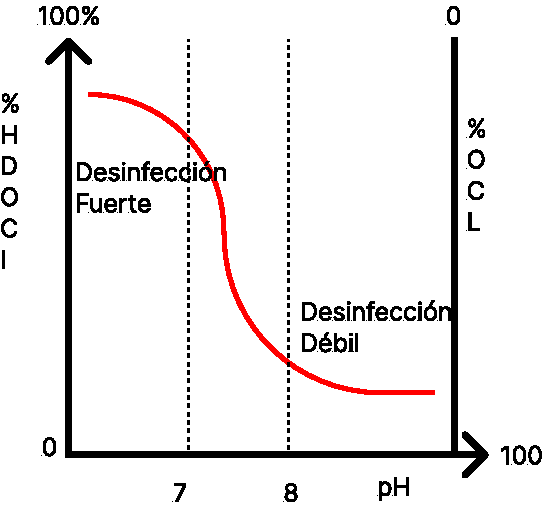
\includegraphics[width=0.5\textwidth]{tusa4.pdf}
  \caption{Diagrama de distribución de cloro}
  \label{tusa4}
\end{figure}
\begin{figure}[h!]
\centering
  \includegraphics[width=0.5\textwidth]{tusa5.jpg}
  \caption{Diagrama de distribución de cloro, completo}
  \label{tusa5}
\end{figure}
\begin{figure}[h!]
\centering
  \includegraphics[width=0.5\textwidth]{tusa6.png}
  \caption{Estabilidad de la solución desinfectante en diversas condiciones.}
  \label{tusa6}
\end{figure}
De la figura \ref{tusa6}, cabe remarcar que el método se lleva en un frasco traslúcido

La pared celular de un microorganismo patógeno es cargado negativamente por naturaleza. Puede ser penetrado por un bajo ácido clórico.

\subsubsection{Cómo el $CLO_2$ mata la bacteria}
Componentes de la célula y sobre la superficie de la membrana celular que contiene material oxidable que reacciona con dióxido 6-7mg/l. clorhídrico, causando la disrupción del metabolismo celular. El dióxido clorhídrico reacciona directamente con los enlaces de disulfuro en lo aminoácidos.

\subsubsection{Demanda de cloro}
El cloro añadida al agua no es necesariamente disponible para la desinfección. Bajas cantidades del agua tiene una demanda de 

El cloro reacciona con amoníaco (punto de quiebre de la cloración), materia orgánica (disuelto y en color) y iones metálicos.

\subsubsection{Cloro combinado}
$Cl_2+NH_3(1-50\,PPM)$, la sustitución secuencial de hidrógeno en amonio sigue como:
$NH_3\implies NH_2Cl\implies NHCl_2\implies NCl_3$. En pH bajo y alto en la relación de $Cl: NH_3$, el $NCHL_2$ y $NCl_3$ se convierte más abundante

$NHCl_2$ es un buen desinfectante pero es asqueroso en el agua.

Alta relación $Cl:NH_3$ también incrementa la relación del punto de quiebre de las reacciones:
\begin{figure}[h!]
\centering
  \includegraphics[width=0.5\textwidth]{tusa7.jpg}
  \caption{Curva del punto crítico de la cloración}
  \label{tusa7}
\end{figure}
Luego del punto crítico del cloro, se convierte en un cloro libre (lista para reaccionar). En ésta muestra de agua depende mucho la cantidad de materia que está disuelta en ella y la dosis de cloro de mg/l variará, aquí fue de 7-8.

\subsubsection{Práctica de cloración}
\textbf{Combinación residual}: cloración marginal simple: aceptable para agua de manantiales. \textbf{Tratamiento de cloro-amonio}: agregando $NH_3$ y $HOCl$ para aguas subterráneas.

\textbf{text} los dos pasos son: punto de quiebre de cloración y supercloración+ decloración ($SO_2, S_2O_3^{2-}$ or carbon activado)

El cloro también reacciona con $H_2S,Fe(II),Mn(II)$ de aguas subterráneas.
\begin{align*}
    &H_2s + \binom{4}{l}_2 + fH_2O\longrightarrow H_2SO_4 + 8HCl\\
    &H_2S + Cl_2\longrightarrow S + 2HCl
\end{align*}
El otro ejemplo es:
\begin{equation*}
    2Fe(HCO_3)_2 + Cl_2 + Ca(HCO_3)_2\longrightarrow 2Fe(OH)_{3(s)} + CaCl_2 + 6CO_2
\end{equation*}
Asociado con el aumento de pH. Es útil para remover metales y producción de coagulantes.
\subsubsection{Problemas de desinfección}
\begin{itemize}
    \item influencias de efectividad del pH
    \item Formación de THM (cancerígenos)
    \item Deformación de la precloración
\end{itemize}
Una alternativa estratégica es reemplazando el $Cl_2$ por otro oxidante o remover los microorganismos por una clarificación más eficiente.

Para la naturaleza de los patógenos, existen factores que influencian la desinfección
\begin{itemize}
    \item Numero y naturaleza de los patógenos
    \item Tipo y concentración de desinfectante
    \item Temperatura (Mayor temperatura, incrementa la tasa de mortalidad)
    \item Tiempo de contacto (mientras más contacto, mayor mortalidad)
    \item Presencia de partículas orgánicas, $H_2S$, reducida a $Fe+Mn$ 
    \item pH
    \item Mezclar la solución para expandir el soluto (cloro)
    \item Demanda de cloro: $NH_3$
\end{itemize}

El ozono es un gas natural ocurrente en la atmósfera de la tierra, es una de los oxidantes naturales más poderosos. En la zona superior de la atmósfera, el ozono filtra los rayos ultravioleta del sol y protege la tierra de una radiación dolorosa, pero en la superficie, el ozono juega un rol en la purificación del agua potable a través del tratamiento de ozono. Es versátil y puede ser empleado comercialmente y en el hogar.

El tratamiento de ozono es un método de tratamiento de 

Cuando la electricidad o rayo ultravioleta incide a través del aire, la energía divide la molécula de oxígeno en dos átomos de oxígeno.
Para perder átomos de oxígeno entonces se recombinan con moléculas de oxígenos ordinarios del ozono.

El ozono reacciona con el hierro, manganeso, sulfuro de hidrógeno y las bacterias o virus.

Las reacciones más simples son dos reacciones de ozono: 

\subsubsection{Remoción del Sulfuro de hidrógeno del agua con ozono}
El Sulfuro de hidrógeno ($H_2S$) crea un olor indeseable en el agua (como a huevos rotos), in aplicación del agua potable, el $h_2S0$ es removido usualmente para potabilizar el agua. La cantidad teórica de ozono requerida para remover H2S es de 3mg de ozono por cada mg $H2S$ El $H2S$ es oxidada a un sulfato y sal soluble

El ozono reacciona con componentes orgánicos; es más difícil predecir la cantidad de ozono requerido para remover materia orgánica del agua. Primero algún componente orgánico no reacciona con ozono, incluso si está expuesta a un oxidante fuerte. Estos componentes son típicamente ácidos carboxílicos, acetonas y aldehídos.

Las proteínas, péptidos y otros aminoácidos de enzimas vitales son rotas en péptidos pequeños a través del procesos de oxidación. Y las grasas polisaturadas son oxidadas a un ácido peróxido. Los microbios son detectados por una disrupción de plasma en las membranas o en el procesos de la desintegración celular. EL ozono también muestra efectividad para desactivar las esporas bacterianas como la liz. Bacillus sp.

Al igual que en el cloro, existen organismos más vulnerables (bacterias) o resistentes (protozoos); 

El promedio la concentración de ozono, multiplicado por el promedio del tiempo de exposición da como resultado el tiempo de contacto.

La relación del volumen del gas a un volúmen líquido (G/L), tiene relaciones bajas en eficiencia. El tamaño de la burbuja, es mayor el área de contacto; La demanda de Ozono del agua, tiene mayor demanda de eficiencia. 

La concentración de ozono, tiene una concentración mayor incrementa la eficiencia; A mayor presión mayor eficiencia, con mayor tiempo de detención también se incrementa la eficiencia y las bajas temperaturas.    

\subsubsection{Mecanismos de desinfección}
Todo depende de la longitud de onda generalmente en un rango de (250-265) para un poder desinfectante, los microbios patógenos fueron generalmente el número de objeto, como resultado es posible diseñar el equipamiento de irradiación ultravioleta para conocer virtualmente cualquier requerimiento de desinfección.

En cualquiera de las longitudes de onda inciden en el material genético, dañando el ADN deshaciendo los enlaces de la doble hélice.

Los 254 nanómetros son la longitud de onda letal de los rayos ultravioleta mediante lámparas de mercurio
\begin{itemize}
    \item Las moléculas T del ADN, en el núcleo del organismo, absorbe la luz ultravioleta
    \item EL organismo es inactivado cuando la dosis suficiente ha sido absorbida para modificar la estructura molecular del ADN
    \item Éste resultado cuando es expuesta causa que dos moléculas de timinas forman un dímero
    \item El efecto de éstos dímeros de timinas causando a lo largo del ADN, cadenas que no pueden replicarse 
\end{itemize}
No existe una dosis exacta, está dada por la intensidad multiplicada por el tiempo de exposición
\begin{equation}
    UV[mW\cdot seg/cm^2]=\text{Intensidad UV}\times \text{Tiempo de Exposición}
\end{equation}
El tiempo de contacto es normalmente de 10-20 segundos, luego con la muestra se hacen diluciones para obtener partes por millón requeridas, para definir el tiempo o concentración de los rayos UV.

% 5 $16000\mu sec/cm2$
% 3 $40000\mu sec/cm2$
% 1.3 $90000\mu sec/cm2$
% Tiempo de residencia hidráulica

Los rayos no serán eficientes cuando:
\begin{itemize}
    \item Haya disoluciones orgánicas
    \item Ácidos húmicos, taninos, o lignina
    \item Presencia de metales
    \item Minerales disueltos tienen un efecto ligero en la eficiencia de la desinfección por UV
\end{itemize}

Mitos de la desinfección de la desinfección UV

Falta del agente residual de desinfección: las bombas, líneas de distribución, pueden ser químicamente desinfectadas a priori para su instalación.

El agua desinfectada entonces fluyendo a través del sistema se mantendrá limpia, también que la radiación ultravioleta no es una método de desinfección feasible para altas tasas de flujo. El costo de capital de los sistemas de rayos ultravioleta tienen una cloración excesiva, pero invariablemente la comparación es invalida. Una inyección de una bomba de alimentación química para algún desinfectante no puede ser comparada con un esterilizador de ultravioleta. Un comparación real debe ser añadida al menos un fuente de carbón para su descloración. Cuando todos éstos factores está en consideración, los rayos ultravioleta es el método más rentable y económico de todos.

\section{Tratamiento de aguas residuales con humedales artificiales}

Se basa en la utilización de plantas emergentes para la depuración de las aguas residuales, reproduciendo artificialmente las condiciones propias de las zonas húmedas naturales.

Las plantas acuáticas emergentes (carrizos, juncos, aneas, etc) son plantas anfibias que se desarrollan en aguas poco profundas, arraigadas al subsuelo:
\begin{itemize}
    \item Presentan una elevada productividad (50-70 toneladas de materia seca/ha*año)
    \item Toleran bien las condiciones de falta de oxígeno que se producen en suelos encharcados, al poseer canales interiores o zonas de aireación (aerénquima) que facilitan el paso del oxígeno hasta las raíces.
\end{itemize}
En 1971 se construyó el primer humedal artificial, empleándose para:
\begin{itemize}
    \item Tratamiento de aguas residuales urbanas e industriales
    \item Tratamiento de aguas de tormenta
    \item Restauración y creación de ecosistemas acuáticos
    \item Deshidratación de lodos.
\end{itemize}
\subsection{Mecanismos de depuración}
\subsubsection{Eliminación de sólidos en suspensión}
Fenómenos de filtración a través del conjunto que forman el sustrato (sobre el que crecen las plantas) y las raíces
\subsubsection{Eliminación de materia orgánica}
\begin{itemize}
    \item Acción de microorganismos (principalmente bacterias) que en estos sistemas presentan actividades y desarrollos muy elevados
    \item Las plantas actúan como sistema de aireación, suministrando a través de sus raíces, el oxígeno necesario para las bacterias que viven en el sustrato, responsables de la degradación aerobia de la materia orgánica
    \item En zonas profundas pueden darse condiciones de ausencia de oxígeno, produciéndose la degradación anaerobia.
\end{itemize}
Eliminación de nitrógeno
\begin{itemize}
    \item Absorción directa por las plantas (250kg/ha*año)
    \item Procesos de nitrificación y desnitrificación que se ven favorecidos por la existencia de zonas aerobias y anaerobias
\end{itemize}
Eliminación de fósforo
\begin{itemize}
    \item Absorción directa por las plantas
    \item Fenómeno de adsorción sobre los componentes del suelo
\end{itemize}
En el caso del fósforo tiene menor importancia la absorción del mismo por las plantas, siendo los fenómenos físico-químicos los que juegan el papel principal en su reducción.
\begin{figure}[h!]
\centering
  \includegraphics[width=0.5\textwidth]{tusa8.png}
  \caption{Esquema general de un HAFS}
  \label{tusa8}
\end{figure}
Consta de un conjunto de balsas con vegetación emergente (aneas, carrizos, juncias, juncos, etc) y niveles de agua pocos profundos (0.1-0.4m)
\begin{figure}[h!]
    \centering
      \includegraphics[width=0.5\textwidth]{tusa9.png}
      \caption{Diagrama de funcionamiento de un HAFS}
      \label{tusa9}
\end{figure}
\subsection{Humedales artificiales de flujo subsuperficial}
En éste tipo de humedales, que se emplean como tratamiento secundario, el agua residual pretratada fluye horizontalmente a través de un medio poroso (gravilla o grava), confinando en un canal impermeable, y en el que se implanta vegetación emergente, generalmente carrizo.
\begin{figure}[h!]
    \centering
      \includegraphics[width=0.5\textwidth]{tusa10.jpg}
      \caption{Humedal subsuperficial}
      \label{tusa10}
\end{figure}
\subsubsection{Humedales artificiales de flujo subsuperficial vertical}
\begin{figure}[h!]
    \centering
      \includegraphics[width=0.5\textwidth]{tusa11.jpg}
      \caption{Humedal subsuperficial vertical y horizontal}
      \label{tusa11}
\end{figure}
























































